% !TeX root=debugging.tex

\subsection{Approaches}

\begin{frame}
    \frametitle{False assumptions}
    \tikz[overlay]\node[anchor=east] at (70ex,8ex) {\tiny\href{https://sway.office.com/PavDhCql8Adms1Ap}{\textit{The Art of Debugging}}, Ehsan Hajyasini, UT AP F96};
    Finding your bug is a process of confirming the many things you believe are true, until you find one which is not true.
    \onslide<+->
    \begin{itemize}[<+->]
        \item you believe that at a certain point in your source file, a certain \textbf{variable} has a certain \textbf{value}
        \item you believe that in a given \texttt{if-then-else} statement, the \texttt{else} \textbf{branch} is the one that is \textbf{executed}
        \item you believe that when you call a certain function, the \textbf{function} \textbf{receives} its \textbf{parameters} correctly
    \end{itemize}
    \onslide<+->So\dots check the assumptions!\onslide<+-> $\longrightarrow$ binary search\onslide<+->, pre \& post conditions
\end{frame}

\begin{frame}
    \frametitle{Stabilize, isolate, minimize}
    \tikz[overlay]\node[anchor=east] at (70ex,14ex) {\tiny\href{https://sway.office.com/PavDhCql8Adms1Ap}{\textit{The Art of Debugging}}, Ehsan Hajyasini, UT AP F96};
    \begin{itemize}[<+->]
        \item make failure-inducing \textbf{input smaller} \onslide<+->$\longrightarrow$ is more relevant\onslide<+->, saves time
        \item make the program \textbf{crash faster}
        \item make the situation \textbf{deterministic} \onslide<+->$\longrightarrow$ make bugs \textbf{reproducible}
    \end{itemize}
\end{frame}

\begin{frame}
    \frametitle{Reproducing bugs}
    \begin{figure}
        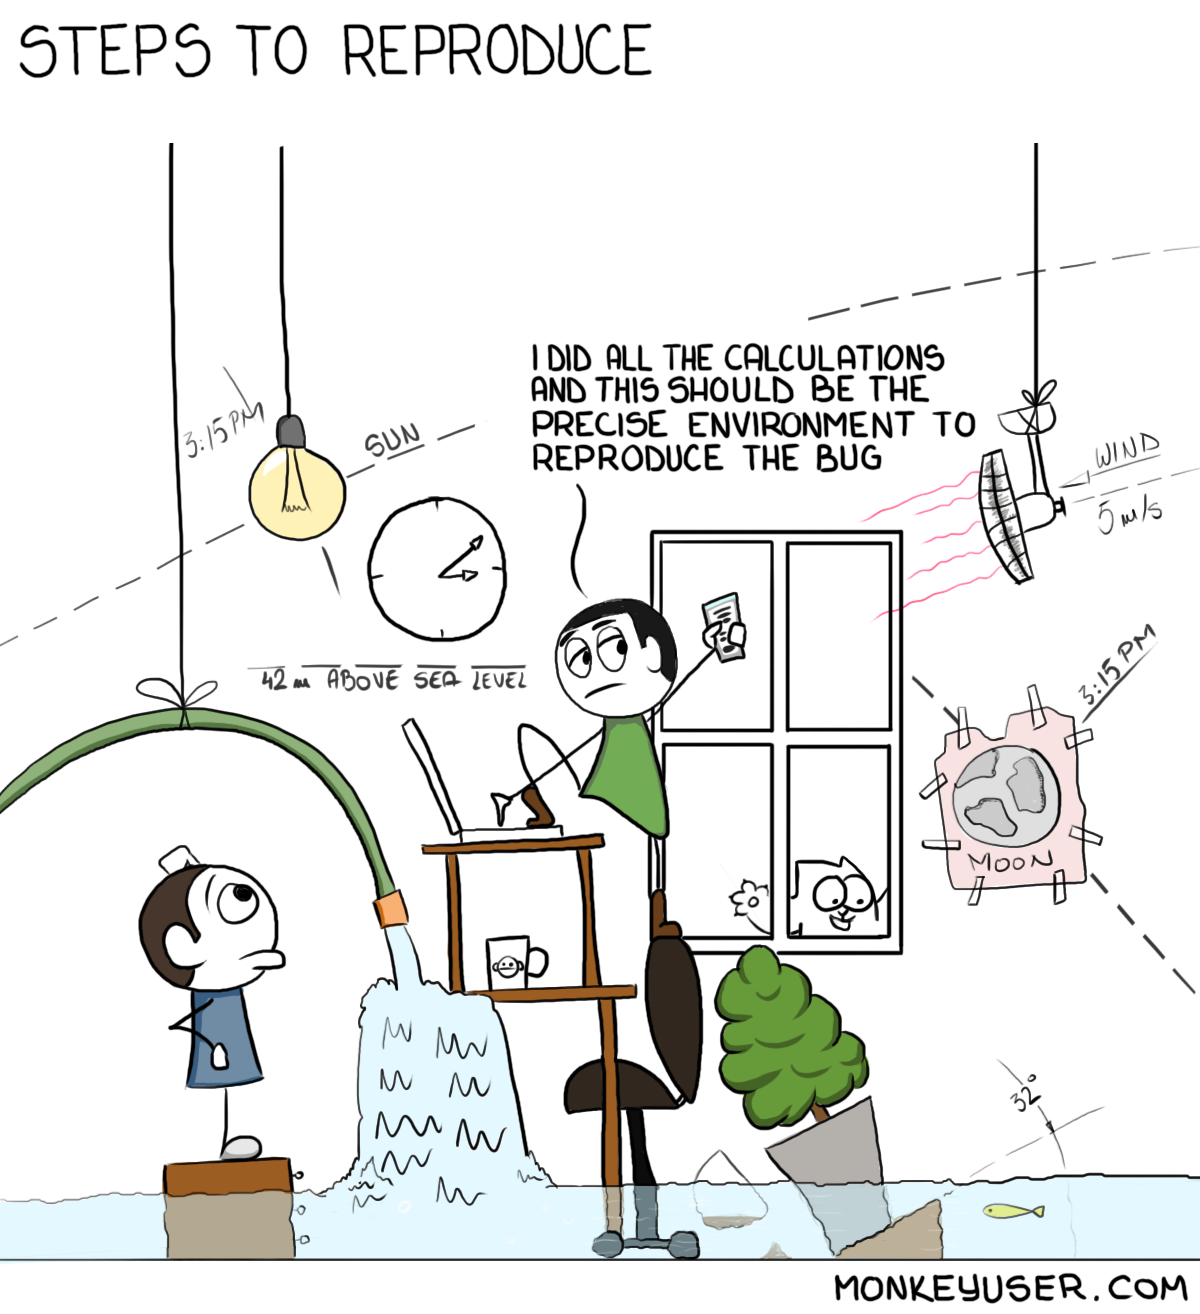
\includegraphics[height=0.8\textheight]{steps-to-reproduce.png}
    \end{figure}
\end{frame}

\begin{frame}
    \frametitle{Scientific method of debugging}
    \tikz[overlay]\node[anchor=east] at (58ex,5ex) {\tiny\textit{Debugging}, Max Goldman and Rob Miller, \href{http://web.mit.edu/6.031/www/fa17/}{MIT Software Construction (6.031) F17}};
    \tikz[overlay]\node[rotate=-6] at (63ex,4.5ex) {
\includegraphics[width=0.13\textwidth]{whyprogramsfail.jpg}};
    \begin{enumerate}[<+->]
        \item \textbf{study the data} \onslide<+->$\longrightarrow$ incorrect results\onslide<+->, failed assertions\onslide<+->, stack traces
        \item \textbf{hypothesize} \onslide<+->$\longrightarrow$ where the bug might be\onslide<+->, or where it cannot be
            \begin{itemize}[<+->]
                \item \textbf{slicing} \onslide<+->$\longrightarrow$ When you have a failure the \textit{slice} for that value consists of the lines of the program that helped compute the bad value.
                \item \textbf{delta debugging} \onslide<+->$\longrightarrow$ difference between successful execution and failing execution\onslide<+->: test cases\onslide<+->, \href{https://martinfowler.com/bliki/DiffDebugging.html}{diff debugging} \& undoing changes 
                \item \textbf{swap components} \onslide<+->$\longrightarrow$ different implementations
            \end{itemize}
            \onslide<+->\textbf{prioritizing hypotheses} \onslide<+->$\longrightarrow$ old, well-tested code vs recently-added code\onslide<+->, library code vs your code
        \item \textbf{experiment} \onslide<+->$\longrightarrow$ devise and run an experiment 
        \item \textbf{repeat}
    \end{enumerate}
\end{frame}

\begin{frame}[fragile]
    \frametitle{Stack trace}
    \begin{Verbatim}[fontsize=\tiny]
Traceback (most recent call last):
  File "./__main__.py", line 154, in <module>
    main()
  File "./__main__.py", line 145, in main
    config = extract_config(config_file_addr)
  File "./__main__.py", line 21, in extract_config
    config = DictWrapper(json.load(f))
  File "/usr/local/Cellar/python/.../3.7/lib/python3.7/json/__init__.py", line 296, in load
    parse_constant=parse_constant, object_pairs_hook=object_pairs_hook, **kw)
  File "/usr/local/Cellar/python/.../3.7/lib/python3.7/json/__init__.py", line 348, in loads
    return _default_decoder.decode(s)
  File "/usr/local/Cellar/python/.../3.7/lib/python3.7/json/decoder.py", line 337, in decode
    obj, end = self.raw_decode(s, idx=_w(s, 0).end())
  File "/usr/local/Cellar/python/.../3.7/lib/python3.7/json/decoder.py", line 353, in raw_decode
    obj, end = self.scan_once(s, idx)
json.decoder.JSONDecodeError: Expecting property name enclosed in double quotes: line 43 column 5 (char 1114)
    \end{Verbatim}
\end{frame}
